\chapter{Parallel Computation with MapReduce}

\section{Vertical and Horizontal Scaling}

Some important computer applications are so large that they would take
unacceptably long to run on conventional computers.  For
example, a personal computer is more than powerful enough
to balance your checkbook, but not for a financial
application that tracks credit card usage in real time to
detect instances of fraud.  The sheer number of credit card
transactions make this application far too intense for a
personal computer.

There are various ways to cope
with problems of scale  in large applications.
The traditional approach is
\index{scaling!vertical}\index{vertical scaling}\emph{vertical scaling},
which means running the
application on a more powerful computer.
This is the easiest solution in terms of software
because the software does not need to change as the machine scales up.
But what happens when the problem gets bigger than any single machine can handle?
For example, maybe a big, fast computer could handle
a billion credit card transactions an hour,
but not a hundred billion.
At some point, the rate at which transactions take place
will overwhelm the available computing technology.

\index{scaling!horizontal}\index{horizontal scaling}\emph{Horizontal scaling}
offers an alternative.  Instead of
running the application in a single computer,
the application is split into smaller
chunks, and each chunk is run on a separate computer.
Ideally, all of the computers involved are similar in most respects
to personal computers, so that the cost of an additional
machine is a small fraction of the overall system cost.
This makes it economically feasible to scale the
hardware platform as the computation requirements increase.
Horizontal scaling has become the de facto
solution for dealing with web services that have to deal
with rapid growth, such as those provided by
Facebook, Google, eBay, Amazon, Netflix, and many others.

The problem with horizontal scaling, however, is that it is
not always easy to split an application into smaller
chunks.  In fact, this is particularly hard when the program
is written using conventional programming languages, such as
C++ or Java. In conventional languages, the program specifies
a sequence of updates to records stored mostly in fast memory.
That makes it difficult to manage multiple computers
working on the computation at the same time because the
cooperating computers need to coordinate their updates.
The coordination problem can sink the effort to make
the computation go faster.
Getting the appropriate data and the right software
components to the right computer
at the right time presents a host of problems.

One advantage of an equation-based software model
is that the different parts of the software are more decoupled
than they are with the conventional approach.
Everything is defined in terms of operators
that, given operands with appropriate data,
can produce results without
interacting with other parts of the software.
For that reason, it does not matter where or when
the operations are performed.
The problems of getting the right data to the right place
remains, but the task of managing a great many small interactions
between different parts of the software is greatly reduced.

The engineers at Google were faced with one of the largest
scaling problems that computing had ever seen,
namely searching the entire, rapidly growing, worldwide web.
To cope with the scale of this problem and its continual growth,
the horizontal scaling approach was the only practical option.
Even though they use mostly conventional programming methods
for most of their software,
they invented and adopted a way to manage large-scale components
with a programming model called \index{MapReduce}MapReduce
that has a lot in common equation-based software models.
Since Google's introduction of MapReduce,
it has been adopted in many other settings.  For
instance, the \index{Apache Foundation}Apache Foundation
implemented \index{Hadoop}Hadoop, an
open-source implementation of MapReduce that you can
download for free to your computer.
Hadoop is widely used in commercial applications and in research.
We will describe the general nature of
MapReduce systems like Hadoop
and explain how the MapReduce framework simplifies the
development of programs that can scale horizontally by
focusing on just two operations: Map and \index{reduce, map}Reduce.

\section{The MapReduce Strategy}

The \index{reduce, map}\index{MapReduce}\textsf{MapReduce} paradigm
is applicable to problems that process
data that can be represented as a sequence of
\index{key/value pair}key/value pairs.
Not all problems lend themselves to this representation,
but Google engineers recognized that many practical
problems do fit in this category.
The following are a few examples.

\begin{quote}
\begin{itemize}
\item \emph{Counting Words in a Document.}  The data in this
case is the collection of words in a document.  It can be
organized as a list of word/count pairs, where the counts
are initially set to one.  Since any word may appear
multiple times in the document, most words will, in the beginning,
occur in more than one word/count pair.
The objective is to produce a list of word/count pairs
in which each word appears only once and the associated
count is the number of occurrences of
the word in the document.

\item \emph{Finding Words that Link to a Webpage.}  The
purpose of this operation is to find the words that are
most commonly used to link to a particular \index{URL}URL.
For example, your name may be the most
common phrase used to link into your Facebook page.
Google uses this kind of information to select which
pages to display for a particular search.
The MapReduce approach applies to this problem.
The data is the
collection of links on the Internet.\footnote{Nobody knows how many
links there are on the internet, worldwide,
but most estimates place it in the trillions,
and some credible estimates place it in the hundreds of trillions. }
Each link can be represented as a word/URL pair,
where the same word may appear in many different pairs.
To figure out which words are most commonly associated with
a particular web address,
this data needs to be reduced to a collection of
URL/word pairs, where each URL will appear once, associated
with the word that is used most often to link to that URL.

\item \emph{Finding Extreme Values.}  Consider
an application that finds the record high or low temperature
for each of the fifty states of the U.S.
The initial data consists of a list of
city/temperature pairs.  There would be one record for each
recorded temperature in a city. It might be one per day,
one per hour, one per minute, or a varying combination,
depending on the city, and the records would extend over
different periods of time for different cities,
a hundred years for some cities, ten years for others,
and so on. So, each city would occur in many different pairs.
The desired outcome is a collection of city/temperature
pairs where each city occurs only once, and the associated
temperature is the highest (or lowest) one in the recorded data.
\end{itemize}
\end{quote}

What all these applications have in common is that data processing
can be split into three different parts, each involving a list of
key/value pairs, and it is possible to process each individual
data record or key/value pair without having to simultaneously
examine all the other records.  For
example, consider the case of finding the highest
temperature ever recorded in each of the fifty states.
The computation could proceed in three stages.
\begin{quote}
\begin{enumerate}
    \item \textbf{Input Data} pairs temperatures with associated sensors.
        Each pair could have a key identifying a
        specific temperature sensor and
        and a value that consists of the city and state where
        the sensor was located, the date the sensor measured
        the temperature, and the temperature on that date.
        For example, the input data may contain the following
        records
        \begin {quote}
        \begin{itemize}
            \item \textsf{KLAR, Laramie, WY, 2009-05-13, 41}
            \item \textsf{KLAR, Laramie, WY, 2009-05-14, 47}
            \item \textsf{KOUN, Norman,  OK, 2009-05-13, 76}
            \item \textsf{KOUN, Norman,  OK, 2009-05-14, 70}
        \end{itemize}
        \hspace*{1cm}$\vdots$
        \end{quote}
        The first column is the key for each record (for example, KLAR),
        and the remaining columns comprise the value. Many
        records may have the same key in the input data because the
        sensor makes many measurements over time.
        The goal is to reduce that to records
        in which each key appears only once,
        associated with the maximum temperature measured by that sensor.
    \item \textbf{Intermediate Data} is used to pass data from
        the Map operation to the Reduce operation. The Map operation
        processes the \emph{input data} and produces key/value pairs
        that make up the \emph{intermediate data}, and the Reduce operation
        processes the intermediate data to create \emph{output data}.
        In this application, the goal is to find the highest temperature
        for each state, so the Map operation could extract
        the state and temperature from each input data record.
        Then, the intermediate records would be state/temperature pairs.
        \begin {quote}
        \begin{itemize}
            \item \textsf{WY, 41}
            \item \textsf{WY, 47}
            \item \textsf{OK, 76}
            \item \textsf{OK, 70}
        \end{itemize}
        \hspace*{1cm}$\vdots$
        \end{quote}
        In general, the Map operation may produce any number of intermediate
        data points for any given input data record, although in this case
        precisely one intermediate record is generated for each input record.
    \item \textbf{Output Data}, the final result of the MapReduce computation,
        is delivered by the Reduce operation.
        In the high-temperature example, this
        corresponds to the maximum temperature recorded for each state, so the
        there would be exactly one record for each state that appeared in the input data.
        \begin {quote}
        \begin{itemize}
            \item \textsf{WY, 115}
            \item \textsf{OK, 120}
        \end{itemize}
        \hspace*{1cm}$\vdots$
        \end{quote}
\end{enumerate}
\end{quote}
As you can see, the data records are largely independent of one another, so the computer
can process the May 13, 2009 temperature entry for Norman, OK without considering the
May 13, 2009 entry for Laramie, WY.  This enables horizontal scaling, because the
different entries can be processed in different machines.
However, this application also shows the need for combining
the entries for a specific key at a later time.  For example,
to find the high temperature record for Oklahoma, it will be
necessary to consider all the entries for Oklahoma at some
point.

The MapReduce paradigm applies well in these kinds of problems.
The \textsf{map} operation, which receives each
of the input key/value pairs, processes the
pair and produces a large number of intermediate
key/value pairs.  These intermediate pairs use keys that may
or may not be completely different than the input keys.
In the word counting example, the intermediate keys may be the same
as the input keys, namely the words that are being counted.
On the other hand, when looking for words that are used to
link to URLs, the input keys are the words, but the
intermediate keys are the URLs. The MapReduce framework leaves
this choice up to the software designer, which is
one of the reasons that MapReduce is widely applicable.

The second step is the \index{reduce, map}\textsf{reduce}
operation, which combines all the entries
for the intermediate keys and
produces zero or more output key/value pairs.  As before, the
output key/value pairs may use the same keys as the
intermediate or input key/value pairs, or they may use
entirely different keys.

For example, consider the problem of counting words in a
document.  Assume that the document has already been
read, and that it has been broken up into key/value pairs
where each key is a word and the value is always one. These
key/value pairs make up the input data for this problem. For
instance, the Gettysburg address could be represented by a
list of key/value pairs using the notation ( \emph{key} ~.~ \emph{value} )
to denote a pair.
\begin{quote}
\begin{itemize}
\item \textsf{( four~.~1 )}
\item \textsf{( score~.~1 )}
\item \textsf{( and~.~1 )}
\item \textsf{( seven~.~1 )}
\item \textsf{( years~.~1 )}\\~~~~$\vdots$
\item \textsf{( from~.~1 )}
\item \textsf{( the~.~1 )}
\item \textsf{( earth~.~1 )}
\end{itemize}
\end{quote}

The map operation takes in an input key and
value, and delivers a list of zero or more intermediate
key/value pairs.  For the word-count program, map could
deliver a list with exactly one element, namely
the very same input key and value.
In this case, the map part of MapReduce
packages the result in a list, which is
the form expected by the MapReduce system,
but does not perform any additional computation.
\begin{displaymath}
map(k, v) = [ ( k ~.~ v ) ]
\end{displaymath}
In a more elaborate example, map would perform
a computation using the key/value pair supplied as
its operand and deliver a list representing the results
of that computation.

The reduce operation accepts an intermediate key and a list of
all the values returned by any map operation for that key.
It delivers a list of zero or more final key/value pairs.
In the case of word-count, reduce returns only one key/value pair,
namely the key and the sum of the counts in the list.
\begin{displaymath}
reduce(k, vs) = [ ( k ~.~ sumlist(vs) ) ]
\end{displaymath}
The operator sumlist, which adds all the elements of its
input, would be defined by the software designer.

To make this discussion more concrete, consider the Gettysburg Address,
which contains the word ``nation'' in four places. Because of this,
the map operation will be called with the input key/value pair \textsf{(nation~.~1)}
four times, and each time it will return a list with
the single intermediate key/value pair \textsf{[(nation~.~1)]}. The MapReduce
system collects all the values for each intermediate key, and starts the reduce
operation on those values.
At some point it will collect all of the four intermediate
values for ``nation'' and invoke the reduce operation with the operands
\textsf{nation} and \textsf{[1 1 1 1]}.
The reduce operation will then
return a list with the final key/value pair \textsf{[(nation~.~4)]}.

% \todo{QUESTION (11/23/17): I don't think this makes sense.
%      Where does vs come from? Earlier, map produced [(k~.~v)].
%      There was no list of vs, just one v. It seems that
%      reduce could create the vs list, but map couldn't supply it
%      a list of vs for each k, but not a list of all the v's
%      associated with a particular k-value. The reduce step
%      could coalesce the duplicate k-values, but that's
%      it wouldn't help much to have reduce sum the v's for
%      non-coalesced k-values.
%      Maybe it would be better to define
%      map(k, v) = v, then explain that the MapReduce
%      system forms a list of all the results produced
%      by map when it operates on the key/value pairs, one by one,
%      then talk about what the reduce step does in this example.
%      Or something.}

Much of the value of MapReduce is that the programmer only needs to
define the map and reduce operations and
does not need to deal with the details of carrying out the map and reduce
operations in a collection of computers sharing the data across a
network.  It is the MapReduce
framework that takes care of running the program in a single
computer, or in a cluster of hundreds or even hundreds of thousands
of computers, depending on the size of the problem.
It also takes care of things like
sending the intermediate key/value pairs
from the computers processing the map operation to the computers
processing the reduce operation.

The MapReduce framework
takes the input key/value pairs and splits them across many
different machines.  On each machine, it performs the map
operation on each of the key/value pairs that is assigned to
that machine.  As it does this, it combines the intermediate
key/value pairs returned by each map operation into a single
list.  The lists from all of the machines are then combined.

The intermediate lists must be combined because
the reduce operation expects to see an intermediate key and all
of the values associated with that key at the same time. For example,
to find the maximum temperature for the key \textsf{OK}, the reduce
task needs to see all the records associated with \textsf{OK}.
Different intermediate keys, such as the ones for \textsf{OK} and \textsf{WY},
are independent, so they can be processed by different machines.
That is, one machine can process \textsf{OK} temperatures at the same
time that another machine is processing \textsf{WY}.
But all of the \textsf{OK} records must go to the same machine running
the reduce operation for \textsf{OK}.
Therefore, the map operation collects all of the values for
each of the intermediate keys, and then the reduce operation is
called only once for each intermediate key.

Once all the values for a given intermediate key are
collected, the MapReduce framework can call the reduce
operation on that intermediate key.  The result is a list of
output key/value pairs. MapReduce collects all these
results and returns them as the final result of the computation.

MapReduce does the work of distributing
the program across multiple machines.
That is one way it provides value.
An engineer can develop a MapReduce program on
a local computer and modify it until it behaves as
required on a small data set.
Then, the program can be submitted to a large MapReduce cluster
to process a full-scale data set.
The MapReduce system deals with the problem of scale
automatically, once the program has been developed.

\section{Data Mining with MapReduce}

\index{data mining}\index{mining, data}Now
that we have seen the basics of MapReduce, we can look at
a larger example that illustrates how MapReduce is
used in practice.  The application we will discuss is a recommendation engine,
a piece of code that is used to recommend new things to a person,
based on other things the person likes.
For example the product page that pops up on a typical visit to
the Amazon website often has a section called ``Customers Who Bought
This Item Also Bought'' that recommends related items.
Based on past purchases and browsing habits, the Amazon software
builds a customized web page full of recommendations.
How does Amazon do this?

Let's break the problem down into
two components.  First, \index{Amazon}Amazon
needs to find \emph{customers like you}.
In the case of a single product, this means other customers who
have bought the product.  In the more general sense,
it means other customers who have bought many
of the same items that you have purchased in the past.
Once the group of
customers like you is identified, the purchases
that people in the group have made can be examined
to find the most popular items.

Finding the most popular items is a problem that is a lot like
counting words in a document.
Amazon keeps a history of all the purchases that each
customer has made.  To process this list with MapReduce, think of it as
consisting of entries of the form customer/item, meaning that at some time the specified
customer bought that particular item.
The map operation produces intermediate entries of the type item/1, meaning
the given item was bought (once),
which is similar to what the word-count program did.
Such an entry should be generated for
each purchase made by a customer in the reference group.  That is,
the map operation filters out the purchases made by customers who are
not like you. The reduce operation is identical to that of word-count,
but this time it counts the number of purchases for each item.
In the end, the computation must consider the results of the reduce operation
and select the items that were purchased most often.

Unfortunately, that leaves the first problem unsolved: finding the group of
customers who are most like you.  This is the most critical aspect for
generating useful recommendations.  For instance, if all of your purchases
from Amazon have been gardening books, you are likely to ignore a
recommendation engine that alerts you to the latest novel in a long-running
vampire series.  Worse, you may start thinking of the recommendations
as unwarranted spam.

How can Amazon find other customers like you?  Imagine that
you have rated all the purchases you have made, giving each item a grade between
0 (hated it) and 5 (loved it).  To keep things simple, imagine that Amazon
sells only two items.  Then your ratings for these items can be expressed as
a pair of numbers, say (2, 0).  Now suppose that other customers have also
rated the items.  The customers who are most like you are the ones
whose ratings are close to yours.
One way to measure how close other ratings are to the pair (2, 0)
is to view the pair
as the coordinates of a point in a two-dimensional plane.
Using this notion of closeness, the customers who
are most like you have purchase histories that correspond to nearby
points in that plane.\footnote{To
determine what points are ``nearby'', you will need
some notion of distance in the plane. You could use the standard,
Euclidean distance or some other distance measurement customized
to the problem of solving the customers-like-you problem.
This is just one of the complex issues that come up
in fashioning methods for finding clusters in data.}

Of course, Amazon sells many more than two items, and neither you nor any
of Amazon's other customers are likely to have rated even a fraction of them.
But the principle stays the same.  Instead of using pairs to represent
ratings, many more coordinates would be needed, as many coordinates
as the number of different products Amazon sells.
The coordinates would still specify a point in space,
but it would be a space with many dimensions.
The customers most like you will still be represented by points close to yours
in that multidimensional space.

A remaining complication is that customers do not always explicitly rate the
items they like, but this can be resolved by using implicit ratings.
For example, if you buy an item, we can give it a rating of 4 unless you
explicitly change it.  And any product that you have never looked at
can be given a rating of 0.

The problem is to find which points in this huge domain with many dimensions
are near your own. Or, viewed another way, the problem is to find groups of
points that are clustered together. One cluster, for example, may consist of
avid gardeners, while another is made up of fans of vampiric fiction.

In general, finding \index{clusters, finding}clusters
in a large data set is a difficult problem
that has been studied extensively
by scientists and mathematicians for a long time.
There are many useful approaches.  One that, on the surface at least,
is straightforward to describe starts with guessing some cluster locations,
then gradually refining the guesses by making computations based on the data.
The computation could proceed as follows.
\begin{quote}
\label{cluster-process}
\begin{enumerate}
    \item Initially, guess a location for each cluster. The guess can be
        taken as the estimated center point of each alleged cluster.
    \item For each point in the data set, decide which cluster center is nearest
        to the point.  Split the points into clusters so that each point is
        in the cluster determined by the nearest center point.
    \item Recalculate each cluster's center point by averaging all the
        points that were assigned to that cluster.
    \item Repeat the previous two steps until things settle down or meet
        some other predetermined conditions.
\end{enumerate}
\end{quote}
The middle two steps can be implemented using MapReduce.  The map operation can
assign points to clusters, and the reduce operation can compute the new center
point of each cluster.  The distances between data points
and estimated cluster centers determines which cluster the data point belongs to,
and the cluster determines the products of interest to particular customers.

The map and reduce operations defined by the programmer
must conform to the expectations of the MapReduce framework.
The framework requires the map operation to be based on
key/value pairs.  In this application, the job of map is
to figure out, for each customer, which cluster center
is closest to that customer's purchase history.
This must be done for all customers, but the MapReduce
framework will take care of distributing the operation across all customers.
We just have to say what the map operation does for an individual customer.

Let's say that the purchase history for the customer is the first operand
of the map operation, and the list of cluster centers is the second operand.
Using this information, the map operation selects the center that is closest
to the customer's purchase history. The MapReduce framework requires the map
operation to deliver its result in the form of a list of key/value pairs,
and we can meet this requirement by specifying that the map operation
delivers a list of just one element, which is a pair consisting of
the selected center (the key) and the purchase history (the value).
\begin{displaymath}
map(hist, centers) = [ ( closest\_center(hist, centers) ~.~ hist ) ]
\end{displaymath}

% \todo{QUESTION (11/23/17): But what is the purpose of v?
%       The result does not seem to depend on it. Is this some kind of
%       symmetry thing, like the symmetry for reduce, below?
%       Needs some kind of explanation.}
The MapReduce framework applies the map operation to all the customers,
gathers up the results, and packages them in the form of
intermediate key/value pairs, one for each cluster center (the key).
The value that the framework associates with the key is the list of
points in the purchase histories associated with the cluster center that
the key represents.
In the equation that defines the map operation,
the center delivered as the key is computed by an operator
called $closest\_center$, which does the work of selecting one
of the centers from the list supplied as its second operand.
The one it selects is, of course, the one that is closest to
the customer history supplied as its first operand.

The $closest\_center$ operation would need to be defined,
and the details depend on how distances between
points are measured. We have deferred deciding those
details, so we will leave that part of the computation
out of the discussion.
In any case, an intermediate key/value pair is a cluster center
(the key) and a list of nearby purchase histories
(the value). Each purchase history is a point for which the
key is the nearest cluster center to that point.
The MapReduce framework sends the intermediate key/value pairs
to the reduce stage of the process.
Now we need to turn our attention to the reduce operation.

The reduce operation receives
an intermediate key/value pair from the MapReduce framework.
The key is the center of a cluster, which is treated by the reduce operation
as an identifier for the cluster.
The value is a list of the points in the cluster.
The job of the reduce operation is to compute a new
center for the cluster (the key) by averaging the list of points (the value).
The MapReduce framework requires the reduce operation to deliver
a list of key/value pairs, so we package its result as a list consisting
of exactly one key/value pair, namely the cluster identifier (the key) and the
new center (the value).
\begin{spacing}{0.9}
\begin{eqnarray*}
    \begin{array}{l@{}l}
        reduce(&cluster, \\
               &points)
    \end{array} &=& [ ( cluster ~.~ average(points) ) ] \\
average(points) &=& avg(points, (0,0), 0) \\
\begin{array}{l@{}l}
    avg(&points, \\
        &sum, \\
        &count)
\end{array} &=&
    \left\{
        \begin{array}{l@{}ll}
            \multicolumn{2}{l}{sum / count} & \mbox{if } points = [~] \\
            avg(& rest(points),             & \mbox{otherwise} \\
                & sum+first(points),        & \\
                & count+1)                  & \\
        \end{array}
    \right.
\end{eqnarray*}
\end{spacing}

We need to explain some of the operators and terms
in the equations that define the reduce operation
because they are not, in all cases, what might be expected.
The \emph{points} variable refers to a list of points,
and each point is a pair of numbers representing product ratings
by a customer.
The operand $(0,0)$ in the equation that defines $average$ is
also a pair of numbers, both zeros in this case.
These zeros serve as a starting point for adding
up the product ratings to make it possible to compute
averages.\footnote{There are only two product ratings
to simplify the example. In practice there would be
many product ratings, so the data item representing
a customer's ratings (and the initial item with the
zeros that start the calculation)
would have many components, each processed in a manner analogous
to the two-component ratings in the example.}

The $sum$ variable is also a pair of numbers.
Therefore, the addition ($+$) and division ($/$) operators
with $sum$ as a left-hand operand are not the usual arithmetic operators.
The formula $sum + point$ denotes $(s_1, s_2) + (r_1,r_2)$,
which stands for the pair $(s_1+r_1, s_2+r_2)$.
Similarly, $sum/count$ denotes $(s_1,s_2)/count$,
which stands for $(s_1/count, s_2/count)$.
The definitions also refer to the operators $first$ and $rest$.
The operator $first$ delivers the first point in the list of points,
and the operator $rest$ delivers all the points in the list
after the first one.

Finally, the equation defining $avg$ selects one of two formulas,
depending on the value of $points$, which is a list.
If the list is empty (that is, if $points = [~]$),
the formula $sum/count$ is selected as the value of $avg$.
If $points$ is not the empty list, the definition selects
a more complicated formula as the value of $avg$.

There is an important subtlety in the way the equations define
the operator $average$ that computes a new center point of a cluster
from points assigned to that cluster in the map stage of the
MapReduce computation.
The work of computing the average is done by the $avg$ operator.
The definition of $avg$ is inductive and
employs a common trick known as tail recursion
that makes computations like averaging much faster.
We think it is worth complicating the discussion
with this technique because the main point
of MapReduce is to be able to compute things quickly.
The \index{tail recursion}\index{recursive}tail recursion
trick avoids supplying, as an operand to another operator,
the value that $avg$ delivers.
This makes the computation
faster because the computer is able to avoid a lot of bookkeeping
that is required when an inductive
invocation is nested in an invocation of another
operator.\footnote{Section \ref{sec:lemmas} discusses an
example illustrating the effectiveness of tail recursion.}

The result of the reduce operation is a new list of center points
in the same format as the initial guess.
That makes the output of the
reduce operation suitable as
the initial guess for additional map computation steps,
which makes it possible for the computer to perform as many
map/reduce cycles as necessary to find clusters.
Figure~\ref{iterative-map-reduce} diagrams the MapReduce
process that we applied to implement the four-part clustering procedure
discussed earlier (page \pageref{cluster-process}).

\begin{figure}
    \begin{center}
%        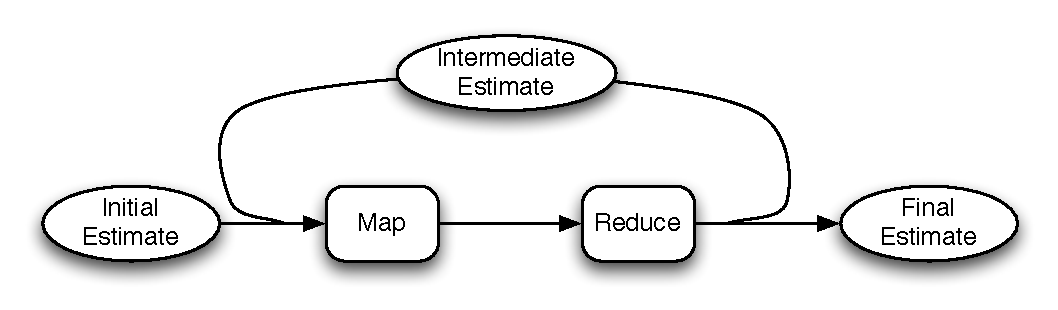
\includegraphics[scale=0.7]{images/iterative-map-reduce}
        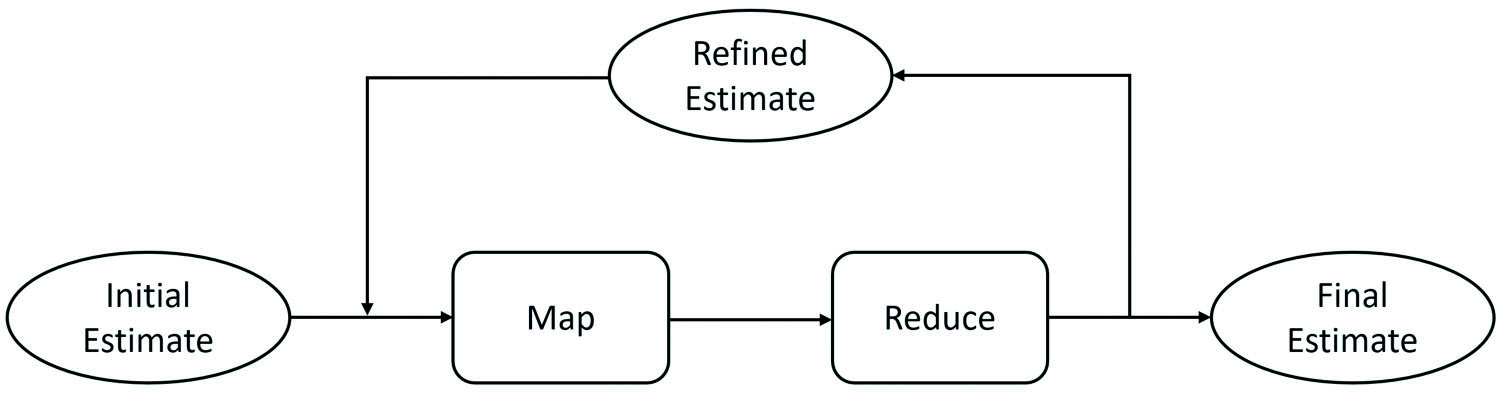
\includegraphics[scale=1]{images-cmyk/iterative-map-reduce-rev}
    \end{center}
    \caption{Iterative Map Reduce Operation}
    \label{iterative-map-reduce}
\end{figure}

\section{Summary}

Some problems are too large to solve on a single, conventional machine.
That leaves two options.
Get a large machine (a supercomputer, for example),
or break the problem down into many tasks and
perform each task on a separate computer.
The first approach,
\index{scaling!vertical}\index{vertical scaling}vertical scaling,
is limited by the size and speed of the most powerful computer available.
In addition it is difficult to use in practice because as the problem grows,
several scaling steps may be necessary,
and each step requires an expensive migration to a more capable computer.
If we were trying to use vertical scaling to deal with the massive,
rapid increases in the volume of traffic on websites
like those of Google and Amazon,
we might need an upgrade every few days,
which would be impossible with vertical scaling.

An alternate approach,
\index{scaling!horizontal}\index{horizontal scaling}horizontal scaling,
offers the promise of virtually unlimited
scalability and incremental increase
in the cost of the solution as the problem size grows.
However, it is much more difficult
to write programs that are split across multiple machines,
and this solution works only
for big computations that can be carried out
in the form of many smaller computations.
Such problems usually involve a lot of data,
and the data needs to be in clumps
that can be processed independently.

\index{reduce, map}\index{MapReduce}MapReduce
is a framework related
to the equation-based software model that facilitates writing
programs that can be distributed across a large number of computers.
MapReduce programs are organized around two operations.
The map operation applies to each of the input values, and
it generates an intermediate result.
The intermediate results are subsequently combined using the reduce operation.
If the results generated by the reduce operation are in the same format
as the input to the map operation, multiple MapReduce passes can be performed.
This is useful in programs that estimate optimal results by refining an initial estimate,
such as programs that find clusters in a large data set.

%%% Local Variables:
%%% mode: latex
%%% TeX-master: "book"
%%% End:
